\documentclass[conference]{IEEEtran}
\usepackage[utf8]{inputenc}
\usepackage[spanish]{babel} 
\usepackage{cite}       
\usepackage{graphicx}       
\usepackage{listings}
\usepackage{xcolor}

%  para mostrar código
\lstset{
    basicstyle=\ttfamily\footnotesize,
    keywordstyle=\color{blue},
    commentstyle=\color{green!60!black},
    stringstyle=\color{red},
    breaklines=true,
    frame=single
}

\title{DSLs y Verificación Formal}

\author{
    \IEEEauthorblockN{Vázquez Dávila José Adolfo \qquad\qquad Cruz Pineda Fernando}
    \IEEEauthorblockA{\textit{Universidad Nacional Autónoma de México}\\
    \textit{Facultad de Ciencias} 
    }
    \IEEEauthorblockA{jose.a\_vazquezd@ciencias.unam.mx \qquad\qquad cruzfernando@ciencias.unam.mx}
}
\begin{document}

\maketitle
\thispagestyle{plain}
\pagestyle{plain}

\begin{abstract}
El álgebra lineal es fundamental en la computación moderna, sin embargo, las bibliotecas estándar suelen verificar la compatibilidad de dimensiones únicamente en tiempo de ejecución, lo que propicia errores tardíos en sistemas. Este trabajo explora cómo los Lenguajes Específicos de Dominio (DSLs) pueden incorporar garantías formales mediante el uso de sistemas de tipos enriquecidos. Se presenta el diseño e implementación de un DSL minimalista para álgebra lineal en Haskell, el cual utiliza tipos fantasma y literales a nivel de tipo para codificar las dimensiones de matrices y vectores como parte de su definición estática. Siguiendo la metodología de verificación de tamaños de Abe y Sumii, el sistema asegura que operaciones algebraicamente inválidas sean rechazadas durante la compilación. Los resultados confirman que este enfoque elimina una clase completa de errores de ejecución, demostrando que un DSL bien diseñado puede proveer verificación formal ligera y corrección por construcción sin requerir herramientas de prueba externas.
\end{abstract}

\section{Introducción}

El álgebra lineal es de suma importancia en el cómputo moderno, aparece en optimización, gráficos por computadora, aprendizaje automático y simulaciones numéricas, entre otros temas. En la práctica, estas aplicaciones se construyen sobre bibliotecas de bajo nivel para operaciones matriciales y vectoriales, donde el programador debe asegurarse manualmente de que las dimensiones de los objetos sean compatibles. Errores tan simples como intentar realizar operaciones entre matrices de tamaños incompatibles suelen detectarse sólo en tiempo de ejecución, cuando la biblioteca ocupada lanza una excepción o, en el peor de los casos, provoca errores de memoria \cite{abe2015}. Trabajos recientes han mostrado que es posible diseñar interfaces de álgebra lineal en las que la compatibilidad de dimensiones se verifica estáticamente mediante el sistema de tipos \cite{abe2015}, reduciendo así toda una clase de errores.


Una forma natural de abordar este problema consiste en recurrir a lenguajes específicos de dominio (Domain-Specific Languages, DSLs). Un DSL es un lenguaje de programación o especificación diseñado para un dominio de aplicación particular, en contraste con los lenguajes de propósito general \cite{mernik2005}. Al sacrificar generalidad, los DSLs pueden ofrecer construcciones más expresivas y cercanas a la notación del dominio, mejorar la productividad de los desarrolladores y, de forma crucial para este trabajo, facilitar el análisis y la verificación de propiedades específicas del problema que modelan \cite{mernik2005}. En contextos industriales, se ha mostrado que un DSL bien diseñado puede integrarse en cadenas de herramientas que generan automáticamente modelos formales para verificadores, haciendo viable la verificación formal en procesos de desarrollo orientados originalmente a pruebas \cite{eakman2015}.

Otra línea complementaria para incorporar garantías formales en el software se basa en el uso de sistemas de tipos enriquecidos. Las teorías de tipos dependientes proporcionan un marco en el que los tipos pueden expresar información precisa sobre los valores —como longitudes, dimensiones o invariantes estructurales— y donde el compilador actúa como verificador de dichas propiedades. Esto ha motivado extensiones de lenguajes de propósito general, como Haskell, hacia formas de tipos dependientes que permitan codificar invariantes de dominio directamente en los tipos de programa \cite{eisenberg2016}. Se han propuesto definiciones generales de teorías de tipos dependientes que unifican distintos sistemas en uso y permiten enunciar metateoremas comunes sobre su buen comportamiento \cite{bauer2020}.En conjunto, estos desarrollos refuerzan la idea de que los sistemas de tipos pueden utilizarse como un lenguaje de especificaciones formales, verificadas de manera estática por el compilador.

Este trabajo es la intersección de dos perspectivas: por un lado, los DSLs para capturar de manera precisa la estructura de un dominio; por otro, los sistemas de tipos como mecanismo para expresar y verificar propiedades formales sobre los programas. Aquí se estudia un caso concreto de la pregunta general de cómo los DSLs pueden incluir garantías formales sobre el dominio que representan. El objetivo es diseñar e implementar un DSL minimal para álgebra lineal básica en el que las dimensiones de matrices y vectores formen parte de los tipos, de modo que sólo las operaciones con dimensiones compatibles sean aceptadas por el compilador. El diseño del sistema de tipos y de la interfaz del lenguaje se basa de manera directa en la propuesta de Abe y Sumii para verificación estática de tamaños en bibliotecas de álgebra lineal \cite{abe2015}, adaptándola a un escenario más pequeño centrado en la multiplicación y combinación de matrices y vectores. Otros trabajos sobre tipos dependientes y programación con tipos avanzados en lenguajes de propósito general, como la tesis de Eisenberg sobre Haskell \cite{eisenberg2016}, se utilizan en este proyecto principalmente como contexto teórico sobre el papel de los tipos como especificaciones, más que como soluciones aplicadas al caso de la multiplicación de matrices. 

\section{Marco teórico}

\subsection{Lenguajes específicos de dominio}

Los lenguajes específicos de dominio (Domain-Specific Languages, DSLs) son lenguajes de programación o de especificación diseñados para abordar problemas dentro de un ámbito de aplicación limitado, en contraste con los lenguajes de propósito general (GPLs) \cite{mernik2005}. De acuerdo con Mernik, Heering y Sloane, un DSL se caracteriza por ofrecer construcciones sintácticas y abstracciones semánticas que reflejan directamente los conceptos de un dominio particular, lo que permite aumentar la expresividad y reducir la brecha entre la forma en que los expertos del dominio razonan sobre los problemas y la forma en que estos se codifican en software \cite{mernik2005}. Esta especialización suele traducirse en programas más concisos, mayor productividad y menor esfuerzo de mantenimiento.

En \cite{mernik2005} se propone además un marco sistemático para decidir cuándo conviene desarrollar un DSL y cómo abordar su diseño. En dicho marco se identifican patrones de decisión que consideran factores como la estabilidad del dominio, la criticidad del software y la complejidad de las soluciones existentes, así como patrones de análisis, diseño e implementación que guían el ciclo de vida de un DSL. Entre los motivos para introducir un DSL aparece de forma explícita la posibilidad de habilitar análisis, verificación, optimización y transformación a nivel de las construcciones del propio dominio, algo difícil de lograr cuando las soluciones se expresan únicamente en un lenguaje de propósito general \cite{mernik2005}. Esta observación es especialmente relevante para el presente trabajo, cuyo objetivo es utilizar un DSL para expresar operaciones de álgebra lineal de forma que ciertas propiedades de dominio —en particular, la compatibilidad de dimensiones— puedan ser garantizadas estáticamente.

\subsection{DSLs y métodos formales}

La relación entre DSLs y métodos formales ha sido explorada en diversos contextos, especialmente en el desarrollo de sistemas críticos \cite{eakman2015}. Un DSL proporciona un nivel de abstracción en el que los modelos de sistema se expresan en términos cercanos al dominio de aplicación; a partir de estos modelos, es posible derivar automáticamente representaciones formales adecuadas para herramientas de verificación, como demostradores de teoremas o verificadores de modelos \cite{eakman2015}. De esta manera, el DSL actúa como una interfaz amigable entre
el programador y las técnicas formales que utilizan
las herramientas de verificación.



Eakman et al.\ describen una metodología en la que aplicaciones desarrolladas con un DSL se traducen de forma en gran medida automática a artefactos formales que pueden ser analizados por herramientas de verificación \cite{eakman2015}. En su enfoque, el uso de un DSL estructurado permite generar más del 90\% del modelo formal sin intervención manual, integrando la verificación formal en procesos de desarrollo originalmente orientados a pruebas \cite{eakman2015}. Este tipo de trabajo muestra una forma concreta de aprovechar un DSL para acercar la verificación formal a sistemas complejos: el DSL no sólo facilita la programación en el dominio, sino que también sirve como punto de partida para derivar especificaciones formales, que luego pueden ser comprobadas con herramientas especializadas.

El presente proyecto adopta una perspectiva complementaria. En lugar de utilizar el DSL como origen de modelos para un verificador externo, las garantías formales se integran directamente en el sistema de tipos del propio lenguaje. Es decir, se busca que ciertas propiedades de dominio sean impuestas por construcción: sólo los programas bien tipados en el DSL deben corresponder a operaciones válidas en el dominio. Esta línea de trabajo se conecta de manera natural con los desarrollos recientes en sistemas de tipos enriquecidos.

\subsection{Sistemas de tipos enriquecidos y tipos dependientes}

Los sistemas de tipos proporcionan un mecanismo para clasificar expresiones y detectar en tiempo de compilación ciertas clases de errores, como el uso inconsistente de operaciones aritméticas o de estructuras de datos \cite{cardelli1996}. En su forma básica, los tipos distinguen entre categorías amplias (enteros, booleanos, funciones, etc.), pero no capturan propiedades más finas de los valores. La investigación en sistemas de tipos enriquecidos ha mostrado, sin embargo, que es posible incorporar información más detallada en los tipos, de modo que estos puedan expresar invariantes sobre la estructura, el tamaño o incluso el comportamiento de los programas \cite{cardelli1996}.


Las teorías de tipos dependientes representan un punto extremo en esta dirección: en ellas, los tipos pueden depender de valores, permitiendo especificar propiedades tales como la longitud de una lista, el tamaño de una matriz o la satisfacción de ciertos invariantes lógicos \cite{bauer2020}. En este marco, los tipos pueden verse como especificaciones formales y la verificación de tipos como una forma de demostración de teoremas \cite{bauer2020,eisenberg2016}. Bauer, Haselwarter y Lumsdaine proponen una definición general de teorías de tipos dependientes que unifica distintos sistemas concretos y establece condiciones bajo las cuales estas teorías exhiben un comportamiento bien estructurado \cite{bauer2020}. Esta formalización proporciona el contexto lógico en el que se inscriben muchos lenguajes y sistemas de prueba modernos. 

En el plano de los lenguajes de programación de propósito general, la tesis de Eisenberg explora cómo extender Haskell hacia una variante dependientemente tipada \cite{eisenberg2016}. Haskell ya incorpora numerosas extensiones de tipos avanzados (GADTs, type families, promoción de tipos, etc.), que permiten simular patrones típicos de los tipos dependientes dentro del lenguaje. Eisenberg sistematiza estas extensiones y propone Dependent Haskell, una versión del lenguaje en la que la frontera entre tipos y valores se difumina y los tipos pueden expresar propiedades mucho más ricas sobre los datos y las funciones \cite{eisenberg2016}. Aunque la tesis no se centra en álgebra lineal ni en la multiplicación de matrices, sí ilustra cómo los sistemas de tipos enriquecidos pueden utilizarse para capturar invariantes de dominio (por ejemplo, longitudes de estructuras) y garantizar que sólo se construyan programas que las respeten.

\subsection{Verificación estática de dimensiones en álgebra lineal}

El álgebra lineal proporciona un ejemplo particularmente natural de propiedad de dominio que se beneficia de un tratamiento estático: la compatibilidad de dimensiones en operaciones entre matrices y vectores. Las bibliotecas tradicionales de álgebra lineal, como BLAS o LAPACK, delegan la verificación de tamaños al programador y, en el mejor de los casos, detectan inconsistencias en tiempo de ejecución \cite{abe2015}. Esto implica que programas bien tipados desde la perspectiva del lenguaje huésped pueden seguir siendo incorrectos desde el punto de vista del dominio al intentar multiplicar matrices de dimensiones incompatibles \cite{abe2015}.


Abe y Sumii abordan este problema proponiendo una interfaz de biblioteca para álgebra lineal en la que las dimensiones de las estructuras se codifican como parámetros de tipo \cite{abe2015}. En su enfoque, los tipos de vectores y matrices adoptan formas como \texttt{'n vec} y \texttt{('m, 'n) mat}, donde \texttt{'m} y \texttt{'n} son parámetros de tipo que representan las dimensiones. Mediante el uso de \emph{phantom types} y mecanismos de generación de tipos frescos, así como del sistema de módulos del lenguaje huésped, logran que las operaciones de alto nivel sólo sean tipables cuando las dimensiones involucradas son compatibles. Como consecuencia, una gran clase de errores de tamaño se detecta en tiempo de compilación: programas que intentan sumar matrices de distinto tamaño o multiplicar matrices con dimensiones incompatibles simplemente no pasan el verificador de tipos \cite{abe2015}.

Aunque la propuesta de Abe y Sumii se presenta como una interfaz de biblioteca, puede interpretarse de manera natural como un DSL embebido para álgebra lineal, en el sentido de que introduce un vocabulario y unas reglas de composición específicas del dominio que están respaldadas por un sistema de tipos cuidadosamente diseñado. Este trabajo constituye el antecedente más directo del proyecto aquí descrito: la idea de que las dimensiones de matrices y vectores formen parte de los tipos y que la compatibilidad de tamaños sea una propiedad verificada estáticamente. El DSL minimal que se desarrollará en las secciones posteriores retoma esta idea y la adapta a un escenario más reducido, con el propósito de estudiar de forma explícita en qué sentido este tipo de diseño tipado proporciona garantías formales sobre la corrección de las operaciones lineales expresadas en el lenguaje.


\section{Delimitación del problema}

La pregunta central de este trabajo —¿cómo pueden los DSLs incluir garantías formales sobre el dominio que representan?— se mantiene sin modificar a lo largo del documento. Lo que sí se acota es el tipo de respuesta que se va a explorar. Como se discutió en el marco teórico, una posibilidad es partir de lenguajes de propósito general y dotarlos de sistemas de tipos cada vez más expresivos, hasta llegar a variantes con tipos dependientes capaces de capturar invariantes complejas del dominio en los propios tipos de programa. La propuesta de Dependent Haskell de Eisenberg \cite{eisenberg2016} es representativa de esta línea: su objetivo es el diseño de un lenguaje general donde los tipos funcionen como especificaciones verificables por el compilador, sin fijarse en un dominio particular como el del álgebra lineal.

En este proyecto se adopta de forma explícita la otra ruta descrita en el marco teórico: partir directamente del dominio y diseñar una interfaz o DSL especializado cuyo sistema de tipos se adapte a las necesidades de ese contexto. En concreto, se toma como referencia la propuesta de Abe y Sumii para verificación estática de tamaños en bibliotecas de álgebra lineal \cite{abe2015} y se la simplifica hasta obtener un DSL minimal centrado en operaciones básicas entre matrices y vectores. No se pretende desarrollar un lenguaje de propósito general con tipos dependientes completos, ni abordar propiedades de dominio más elaboradas (como estabilidad numérica u optimizaciones de rendimiento); el foco se restringe a un único aspecto bien delimitado: garantizar estáticamente la compatibilidad de dimensiones en las operaciones lineales expresadas en el DSL.

\section{Implementación}

La implementación del DSL de álgebra lineal se desarrolló en \textit{Haskell}, siguiendo el enfoque propuesto por Abe \& Sumii (2019) para la verificación estática de tamaños mediante tipos fantasma y literales de tipo. El sistema se organizó modularmente en cuatro unidades funcionales: \texttt{Tipos}, \texttt{Operaciones}, \texttt{DSL} y \texttt{Main}. Esta estructura permite una clara separación entre el diseño de tipos, la semántica operacional y los casos de uso del lenguaje.

\textbf{Módulo \texttt{Tipos}.} Define el tipo central \texttt{Matrix r c a}, donde los parámetros \texttt{r} y \texttt{c} representan filas y columnas a nivel de tipo mediante la extensión \texttt{DataKinds}. La función \texttt{fromList} actúa como constructor seguro, validando en tiempo de ejecución que las dimensiones declaradas coincidan con las del valor proporcionado. La función \texttt{identity} implementa la matriz identidad, garantizando su carácter cuadrado por el sistema de tipos.

\begin{lstlisting}[language=Haskell, caption={Constructor seguro \texttt{fromList} del módulo Tipos.}, label={lst:fromlist}]
fromList :: forall a (r :: Nat) (c :: Nat). [[a]] -> Maybe (Matrix r c a)
fromList xs
  | length xs == r && all ((== c) . length) xs = Just (Matrix xs)
  | otherwise = Nothing
  where
    r = fromIntegral (natVal (Proxy :: Proxy r))
    c = fromIntegral (natVal (Proxy :: Proxy c))
\end{lstlisting}

\textbf{Módulo \texttt{Operaciones}.} Contiene las operaciones elementales (\texttt{add}, \texttt{mul}, \texttt{transposeM}) y extendidas (\texttt{trace}, \texttt{dot}, \texttt{norm}, \texttt{det}). Las firmas de tipo reflejan explícitamente las restricciones dimensionales: por ejemplo, la multiplicación \texttt{mul :: Matrix r m a -> Matrix m c a -> Matrix r c a} sólo se admite cuando las columnas de la primera matriz coinciden con las filas de la segunda. Este diseño traslada las reglas algebraicas al nivel de tipos, evitando operaciones inválidas desde la compilación.

\begin{lstlisting}[language=Haskell, caption={Implementación de \texttt{mul} con verificación estática de dimensiones.}, label={lst:mul}]
mul :: Num a => Matrix r m a -> Matrix m c a -> Matrix r c a
mul (Matrix a) (Matrix b) =
  Matrix [[ sum $ zipWith (*) fila col | col <- transpose b ] | fila <- a]
\end{lstlisting}

\textbf{Módulo \texttt{DSL}.} Define la sintaxis declarativa \texttt{LinExpr r c a}, que modela expresiones algebraicas tipadas. El evaluador \texttt{eval} proporciona la semántica operacional, interpretando las expresiones como operaciones sobre matrices concretas. Así, el lenguaje puede emplearse tanto de forma declarativa (construyendo expresiones) como imperativa (ejecutando operaciones directas).

\begin{lstlisting}[language=Haskell, caption={Evaluador \texttt{eval} que interpreta expresiones algebraicas tipadas.}, label={lst:eval}]
eval :: (Floating a, Num a) => LinExpr r c a -> Matrix r c a
eval (Const m) = m
eval (AddE e1 e2) = add (eval e1) (eval e2)
eval (MulE e1 e2) = mul (eval e1) (eval e2)
eval (TransposeE e) = transposeM (eval e)
eval (DetE e) = Matrix [[det (eval e)]]
eval (TraceE e) = Matrix [[trace (eval e)]]
\end{lstlisting}

\textbf{Módulo \texttt{Main}.} Contiene ejemplos de uso que demuestran la verificación estática. Por ejemplo, la operación \texttt{mul (Matrix 2x3) (Matrix 3x2)} compila correctamente, mientras que una multiplicación incompatible genera un error de tipo en tiempo de compilación. Esta propiedad constituye la base de la \textit{verificación por construcción}, donde el sistema de tipos actúa como especificación formal ligera.

\section{Resultados}

Los resultados obtenidos demuestran que el DSL de álgebra lineal implementado cumple con el objetivo principal de garantizar la corrección dimensional de las operaciones en tiempo de compilación. Las pruebas se realizaron tanto mediante la ejecución del programa principal (\texttt{Main}) como de forma interactiva en el intérprete \texttt{GHCi}, confirmando el comportamiento esperado del sistema de tipos.

En la Figura~\ref{fig:exec1} se muestra la salida del programa ejecutado desde la terminal. Se observa la correcta multiplicación de dos matrices compatibles de dimensiones $(2\times3)$ y $(3\times2)$, obteniendo una matriz resultante $(2\times2)$. Asimismo, el DSL calcula con precisión operaciones adicionales, como el determinante y la traza de una matriz cuadrada, así como el producto punto y la norma vectorial. Los resultados impresos confirman la validez numérica de las operaciones y la consistencia del modelo algebraico definido a nivel de tipos.

\begin{figure}[h]
  \centering
  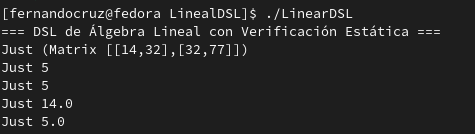
\includegraphics[width=0.85\linewidth]{imagenes/ejecucion1.png}
  \caption{Ejecución del programa principal mostrando operaciones tipadas válidas.}
  \label{fig:exec1}
\end{figure}

Por otro lado, la Figura~\ref{fig:exec2} evidencia el mecanismo de verificación estática de tipos durante el uso interactivo del lenguaje en \texttt{GHCi}. Al intentar realizar una multiplicación entre matrices incompatibles, el compilador genera un error de tipos en tiempo de compilación, indicando que las dimensiones no coinciden (\textit{``Couldn't match type ‘3’ with ‘2’''}). Este resultado demuestra la capacidad del sistema para prevenir errores estructurales antes de la ejecución, validando el principio de \textit{correctness by construction}.

\begin{figure}[h]
  \centering
  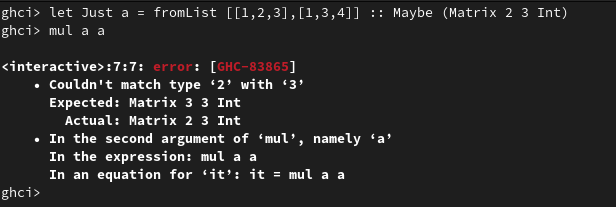
\includegraphics[width=0.8\linewidth]{imagenes/error_tipos.png}
  \caption{Error de verificación de tipos en \texttt{GHCi} al intentar una operación inválida.}
  \label{fig:exec2}
\end{figure}

En conjunto, estas pruebas confirman que el DSL proporciona una verificación formal ligera integrada al propio sistema de tipos de \textit{Haskell}, logrando resultados correctos y consistentes sin necesidad de pruebas externas.

\section{Conclusión}

Como pudimos ver con esta implementación mínima, los DSLs pueden incorporar garantías formales sobre el dominio que representan al integrar en su diseño mecanismos de verificación basados en el sistema de tipos. En lugar de depender exclusivamente de pruebas o validaciones externas, un DSL puede codificar las propiedades invariantes del dominio —como las reglas algebraicas o las restricciones dimensionales— directamente en su semántica y en sus tipos. En el caso del DSL de álgebra lineal desarrollado, el uso de tipos dependientes en \textit{Haskell} permitió que la compatibilidad de dimensiones se verificara en tiempo de compilación, garantizando la corrección estructural de las operaciones por construcción. Este enfoque demuestra que la formalización del dominio en el propio lenguaje no sólo mejora la seguridad y confiabilidad del software, sino que constituye una forma práctica de verificación formal ligera, donde los errores conceptuales se previenen mediante el diseño mismo del lenguaje.

\bibliographystyle{IEEEtran} 
\bibliography{ref}  

%Hay mucha mas informacion que se podría añadir: dsl vs APIS
%DSL no está hecho para ser ejecutable
%indagar en detalles de diseño (seccion 2.4 de la referencia [2])



\end{document}